%!TEX root = ../thesis-summary.tex

\section{Evaluation}
\label{section:evaluation}

As part of our implementation, we needed a way to test our Pulsarcast system.
However we had a set of specific requirements that made our choice of tools
harder. We needed something that fulfilled the following:

\begin{itemize}
  \item Easily deploy and test different versions of our module.
  \item Run tests not only on Pulsarcast but also on IPFS' own pub-sub
    implementation.
  \item Able to extract relevant usage metrics.
  \item Simulate network constraints such as latency.
  \item Able to run locally but easily scalable to a large network.
  \item Can be controlled from a central point, while being able to interact
    with specific nodes in the system.
  \item Easy to create scripts for, so that we could automate as much of our
    test suite as possible.
\end{itemize}

To achieve this we relied on containers, specifically
Docker~\footnote{\url{https://www.docker.com/products/container-runtime}}
containers, which we used to create a containerised version of our module. To
orchestrate our containerised application we used
Kubernetes~\footnote{\url{https://kubernetes.io/}}, an open source
orchestration platform based on Google's learnings on running containerised
workloads at scale~\footnote{\url{https://research.google/pubs/pub43438/}}, and
one of the most popular solutions in the field.

To aggregate, correlate and analyse metrics and logs we used
Elasticsearch~\footnote{\url{https://www.elastic.co/products/elasticsearch}},
Beats~\footnote{\url{https://www.elastic.co/products/beats}},
Logstash~\footnote{\url{https://www.elastic.co/products/logstash}} and
Kibana~\footnote{\url{https://www.elastic.co/products/kibana}}. In order to
simulate abnormal network conditions we relied on
Toxiproxy~\footnote{\url{http://toxiproxy.io}}, a TCP proxy that,
programatically through an HTTP API, allowed us to inject multiple kinds of
faults.

As we know it, Pulsarcast is just a module that applications can use to build
on top of. In order to test it we created a fork of JS
IPFS~\footnote{\url{https://github.com/jgantunes/js-ipfs}} where we integrated
Pulsarcast. This not only provided us with a command line interfaace (CLI) and
an HTTP API to interact with our system, but it also gave us direct access to
IPFS' own pub-sub module, Floodsub, to which we wanted to compare our module.

Figure \ref{fig:ipfs-testbed-and-metrics} provides an architectural overview of
our system. All of the projects and code we created for the testbed are
open
source~\footnote{\url{https://github.com/JGAntunes/helm-charts/tree/master/ipfs-testbed}}~\footnote{\url{https://github.com/JGAntunes/ipfs-testbed}}~\footnote{\url{https://github.com/JGAntunes/ipfs-testbed-cli}}.

\begin{figure}[!htb]
  \centering
  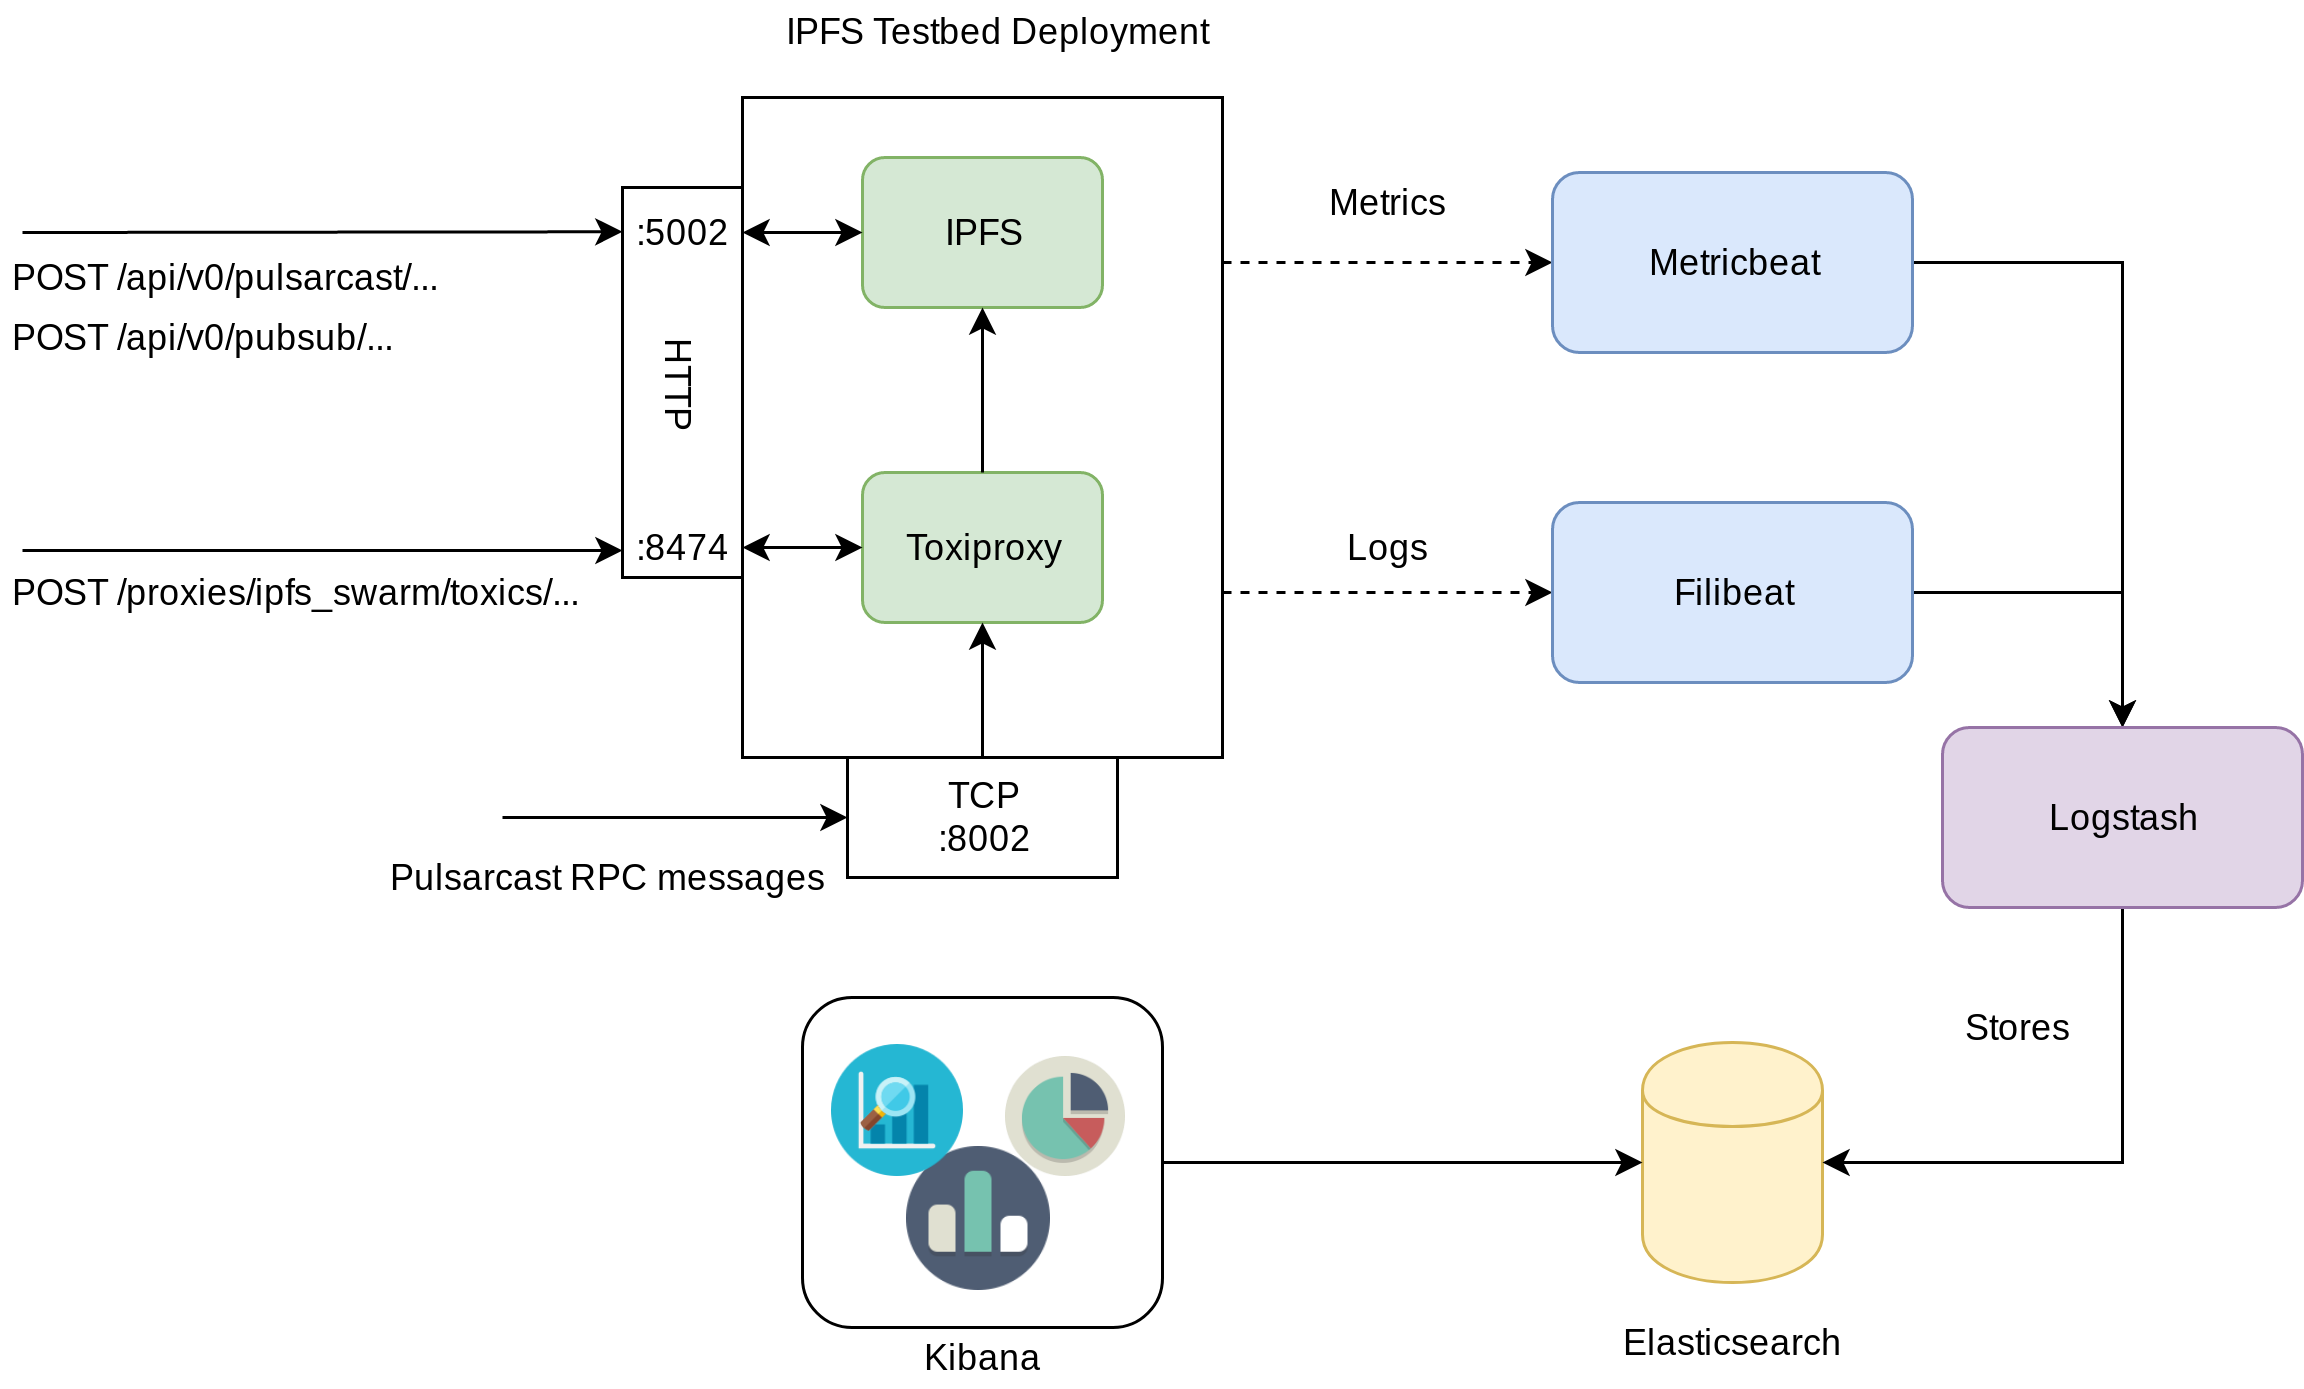
\includegraphics[width=0.45\textwidth]{img/ipfs-testbed-and-metrics.png}
  \caption{Overview of our ipfs-testbed deployment and our metrics/logs
  pipeline}
  \label{fig:ipfs-testbed-and-metrics}
\end{figure}

Our whole setup consisted of a total of 5 VMs~\footnote{Special thanks to
Microsoft and the Azure team for supporting our efforts and offering us free
credits} acting as Kubernetes Worker nodes, each with two vCPUs, 16 GiB of RAM
and 32 GiB of storage. In our cluster, besides other operational bits, we ran 3
Elasticsearch instances, 1 Logstash instance, 1 Kibana and a total of 100 IPFS
Testbed deployments (as described aboe). Because we wanted to avoid resource
starvation and to better take advantage of the Kubernetes scheduler, our
testbed deployments allocate 440 MiB of memory per deployment, each burstable
to a maximum of 500 MiB. During our whole test execution, periodic HTTP health
checks (part of the Kubernetes platform) make sure our deployments are working
accordingly.

To test our system accordingly, we wanted a dataset that could simulate a
real-life scenario as much as possible. We chose to use a dataset of
Reddit's~\footnote{\url{https://www.reddit.com/}} comments from
2007~\footnote{\url{http://academictorrents.com/details/7690f71ea949b868080401c749e878f98de34d3d}}~\footnote{\url{https://www.reddit.com/r/datasets/comments/3bxlg7/i_have_every_publicly_available_reddit_comment/}}
consisting of a sample of approximately 25000 comments in a total of 23 topics
(known as subreddits in the platform)~\footnote{\url{https://github.com/JGAntunes/pulsarcast-test-harness}}.

The following graphs give us a distribution analysis of events published per
topic (Figure \ref{fig:events-to-be-publisher-per-topic}) and subscriptions per
topic (Figure \ref{fig:subscriptions-per-topic}). Given our dataset choice, we
aimed for a non-uniform subscription distribution per topic and, as it would be
expected in a real-world scenario, the distribution of events follows a power
law based on their popularity. 

\begin{figure}[!htb]
  \centering
  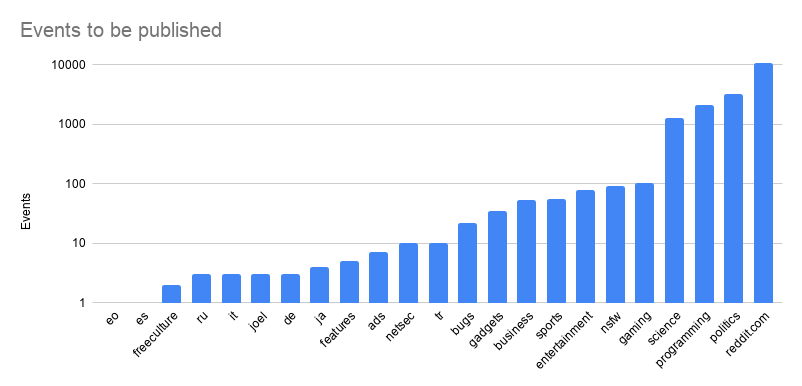
\includegraphics[width=0.35\textwidth]{img/events-to-be-publisher-per-topic.png}
  \caption{Event distribution per topic with log scale}
  \label{fig:events-to-be-publisher-per-topic}
\end{figure}

\begin{figure}[!htb]
  \centering
  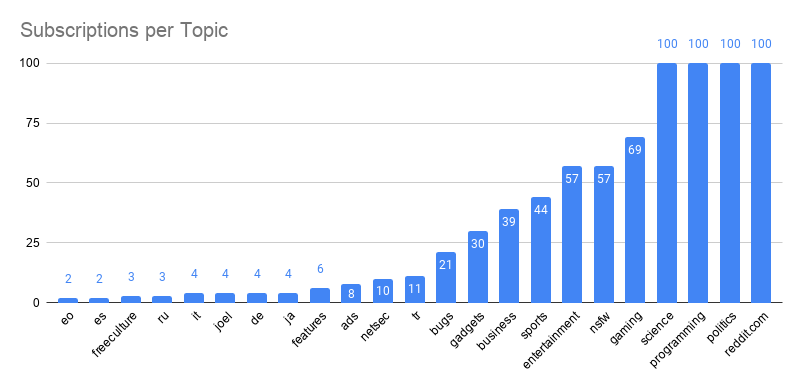
\includegraphics[width=0.35\textwidth]{img/subscriptions-per-topic.png}
  \caption{Subscription distribution per topic}
  \label{fig:subscriptions-per-topic}
\end{figure}

For each execution, we look to extract two key groups of data: resource usage
data and QoS data. The following list describes these in more detail:

\begin{itemize}
  \item Resource usage as a total in the whole cluster, and per-node (95/99
  percentile and average)
  \begin{itemize}
    \item CPU Usage (CPU number)
    \item Memory Usage (GiB)
    \item Network Usage (MiB transmitted)
  \end{itemize}
  \item QoS
  \begin{itemize}
    \item Events published by topic and in total
    \item Events received by topic and in total
    \item Percentage of subscriptions fulfilled based on the number of events
    successfully published
    \item Percentage of subscriptions fulfilled based on the total number of events
    injected in the system
    \item Number of RPC messages sent per topic and in total
    \item Average, standard deviation and percentiles (99/95) of the number of RPC messages received and sent by each node
  \end{itemize}
\end{itemize}

We measure the subscription coverage (number of subscriptions fulfilled)
through two distinct metrics. The percentage of fulfillment having the number
of events effectively published as a reference and the percentage of
fulfillment having the total number of events injected into the system as
reference. Given Pulsarcast's nature, when an event is injected into the
system, depending on the topic configuration, it may need to be propagated
through the dissemination trees before being effectively published
(\emph{request to publish}). It also needs to be persisted in the DHT. Having
two different metrics allows us to better analyse and distinguish the different
behaviours of the system.

Some of the metrics under the QoS group only make sense in Pulsarcast test
runs, hence will be ignored when running the baseline Floodsub solution.

We ran 3 different scenarios under 2 different sets of network conditions to an
effective total of 6 different executions. For each of the 3 different
scenarios we executed one under normal/undisturbed network conditions and
another using Toxiproxy's features, adding a latency of 500 milliseconds and
300 milliseconds of jitter to every incoming TCP packet. The scenarios we ran
were the following:

\begin{itemize}
  \item Pulsarcast without order guarantee (basic usage, every node can publish to any topic)
  \item Floodsub (IPFS' pub-sub implementation)
  \item Pulsarcast with order guarantees (only one node per topic is allowed to publish and all nodes can request to publish)
\end{itemize}

For Pulsarcast without order guarantee our fultilment results were the following:
\begin{itemize}
\item Under normal network conditions
\begin{itemize}
  \item 99\% of subscription coverage, having all the events injected into the system as reference
  \item 99\% of subscription coverage, having the events effectively published as reference
\end{itemize}
\item Under abnormal network conditions
\begin{itemize}
  \item 51\% of subscription coverage, having all the events injected into the system as reference
  \item 86\% of subscription coverage, having the events effectively published as reference
\end{itemize}
\end{itemize}

Figures \ref{fig:graph-pulsarcast-event-fulfillment-comparison},
\ref{fig:graph-pulsarcast-event-percentage-fulfillment-comparison} and
\ref{fig:graph-pulsarcast-latency-event-percentage-fulfillment-comparison} show
us a comparison of event fulfilment rates across topics. A couple of factors
contributed to the discrepancy between the values of the first and the second
executions. The first one is an implementation detail in our Javascript
Pulsarcast module, where on each command it receives, it waits on the initial
DHT persistence and propagation of events/topics before returning control to
the caller (and consequently replying to the clients of our HTTP API). This
creates a natural back pressuring system that ended up dragging the second
execution for 13h versus the 85 minutes that took for the first execution. The
long execution ended up putting a lot of pressure in our testbed which
terminated two Pulsarcast nodes due to resource limitations. Nevertheless, our
fulfilment rates are almost perfect for the first execution and still
considerably high under abnormal network conditions. As for resource usage our
first execution had a maximum memory consumption of 31.924 GiB across the
cluster, with an average of 0.319 GiB per node and a P99 of 0.378 GiB. For the
second execution our memory footprint was fairly higher (responsible for the
node terminations), with a total consumption of 35.8 GiB, average of 0.36 per
node and a P99 of 0.43 GiB. As expected, given our systems were mostly idle,
CPU usage was much lower in the second execution, between 3.5 and 3.8 vCPUs in the
first test run and 0.6 and 1.25 in the second one.

\begin{figure}[!htb]
  \centering
  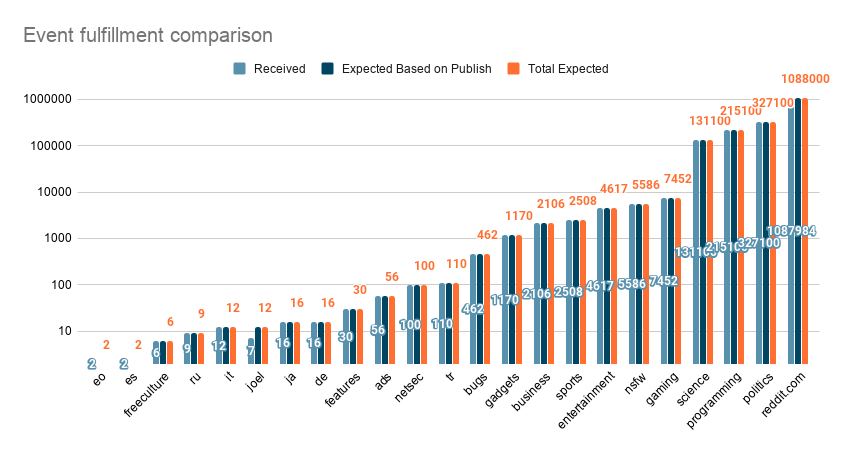
\includegraphics[width=0.4\textwidth]{img/graph-pulsarcast-event-fulfillment-comparison.png}
  \caption{Pulsarcast without order guarantee - Comparison of events fulfilled by topic in a log scale}
  \label{fig:graph-pulsarcast-event-fulfillment-comparison}
\end{figure}

\begin{figure}[!htb]
  \centering
  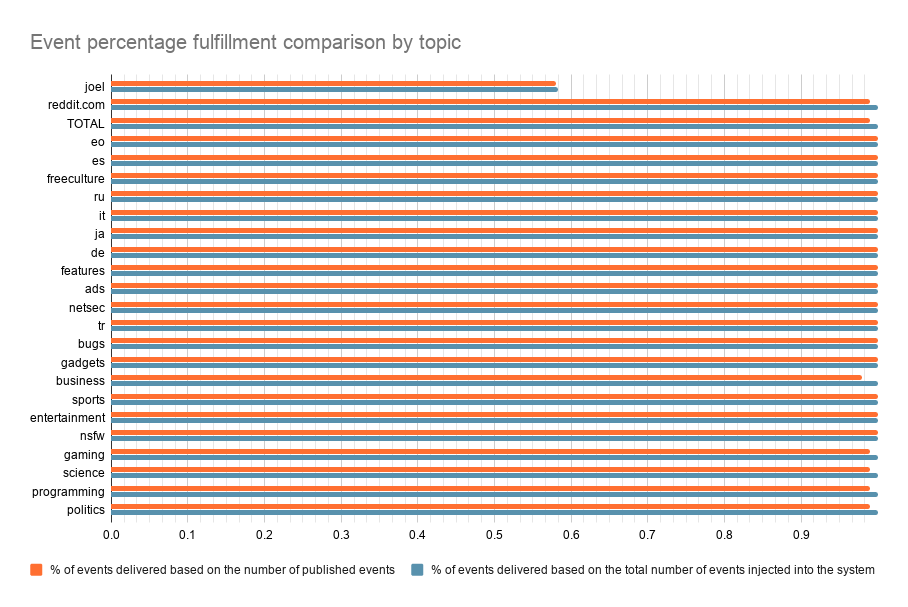
\includegraphics[width=0.4\textwidth]{img/graph-pulsarcast-event-percentage-fulfillment-comparison.png}
  \caption{Pulsarcast without order guarantee - Comparison of percentage of events fulfilled by topic}
  \label{fig:graph-pulsarcast-event-percentage-fulfillment-comparison}
\end{figure}

\begin{figure}[!htb]
  \centering
  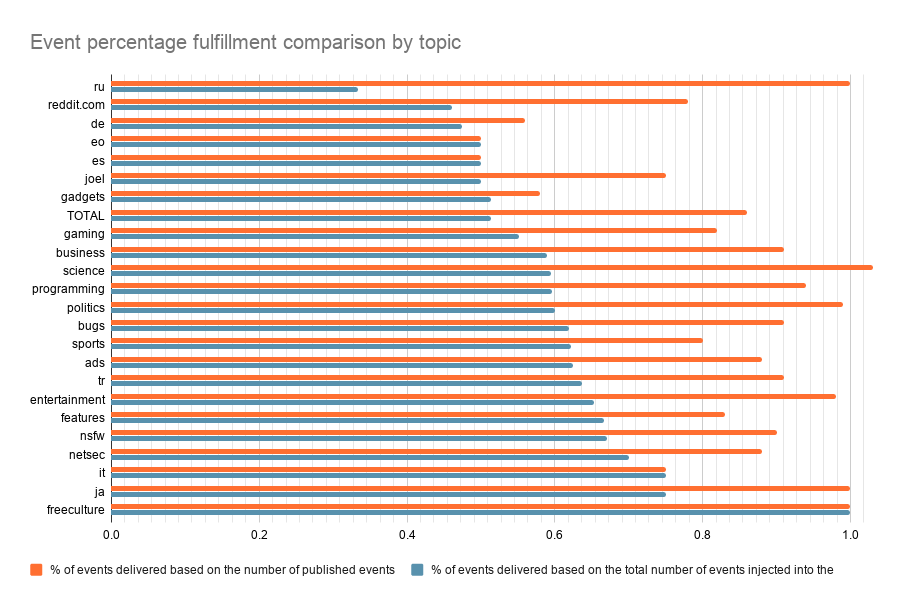
\includegraphics[width=0.4\textwidth]{img/graph-pulsarcast-latency-event-percentage-fulfillment-comparison.png}
  \caption{Pulsarcast without order guarantee and latency - Comparison of percentage of events fulfilled by topic}
  \label{fig:graph-pulsarcast-latency-event-percentage-fulfillment-comparison}
\end{figure}

For Pulsarcast with order guarantee our fultilment results were the following:
\begin{itemize}
\item Under normal network conditions
\begin{itemize}
  \item 37\% of subscription coverage, having all the events injected into the system as reference
  \item 80\% of subscription coverage, having the events effectively published as reference
\end{itemize}
\item Under abnormal network conditions
\begin{itemize}
  \item 32\% of subscription coverage, having all the events injected into the system as reference
  \item 62\% of subscription coverage, having the events effectively published as reference
\end{itemize}
\end{itemize}

Figures \ref{fig:graph-pulsarcast-order-event-fulfillment-comparison},
\ref{fig:graph-pulsarcast-order-event-percentage-fulfillment-comparison} and
\ref{fig:graph-pulsarcast-order-latency-event-percentage-fulfillment-comparison} show
us a comparison of event fulfilment rates across topics. Both executions saw 2
nodes being terminated due to limitations on the resources available to the
testbed, specifically CPU. These executions put a lot of stress into the root
nodes of the most popular topics. Consequently, this affected our fulfilment
rates. However, we are aiming at a total different level of QoS in this
scenario, so it is important to put these numbers into perspective, as it is
unfair to compare them directly with any of the other results in this document.
It is interesting to see though that, despite the added network latency in the
second execution, our QoS did not suffer a clear impact. As for resource usage
our first execution had a maximum memory consumption of 17.84 GiB across the
cluster, with an average of 0.178 GiB per node and a P99 of 0.207 GiB. For the
second execution our memory footprint was quite similar, with a total
consumption of 19.99 GiB, average of 0.2 per node and a P99 of 0.35 GiB. As
expected, given our systems were mostly idle, CPU usage was much lower in the
second execution, between 3 and 4.5 vCPUs in the first test run and 0.93 and
4.33 in the second one.

\begin{figure}[!htb]
  \centering
  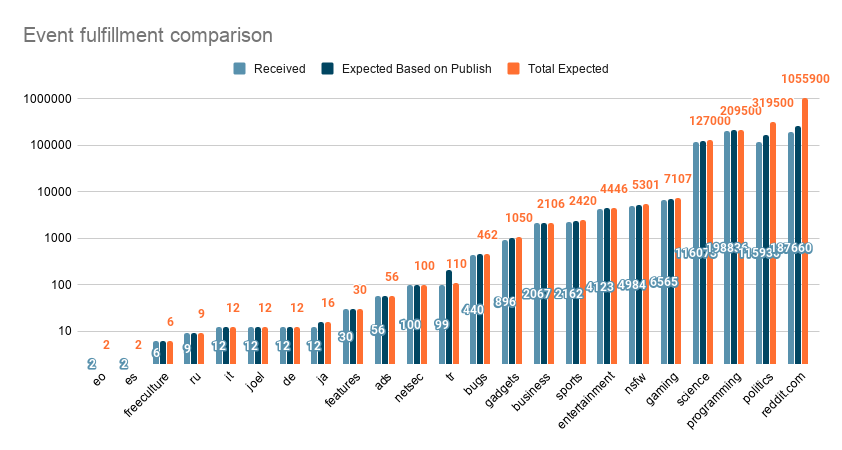
\includegraphics[width=0.4\textwidth]{img/graph-pulsarcast-order-event-fulfillment-comparison.png}
  \caption{Pulsarcast with order guarantee - Comparison of events fulfilled by topic in a log scale}
  \label{fig:graph-pulsarcast-order-event-fulfillment-comparison}
\end{figure}

\begin{figure}[!htb]
  \centering
  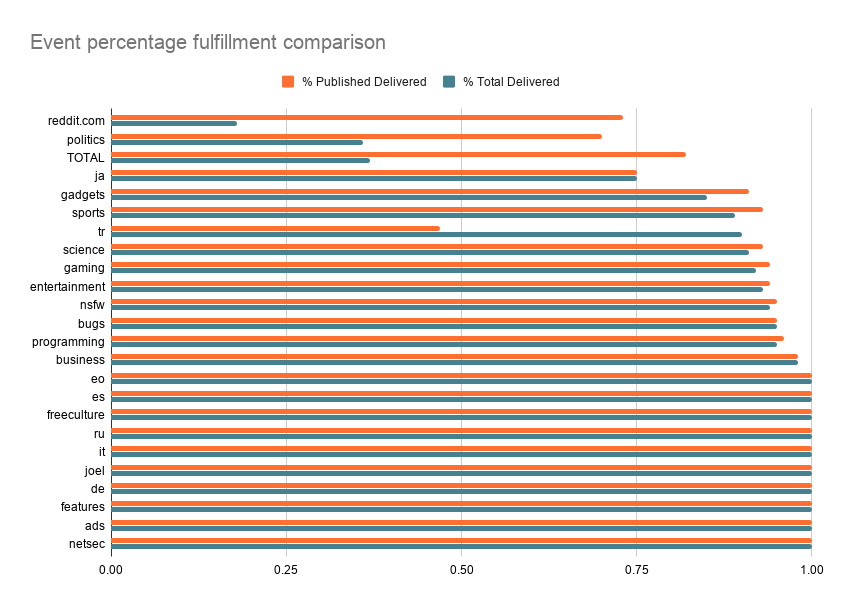
\includegraphics[width=0.4\textwidth]{img/graph-pulsarcast-order-event-percentage-fulfillment-comparison.png}
  \caption{Pulsarcast with order guarantee - Comparison of percentage of events fulfilled by topic}
  \label{fig:graph-pulsarcast-order-event-percentage-fulfillment-comparison}
\end{figure}

\begin{figure}[!htb]
  \centering
  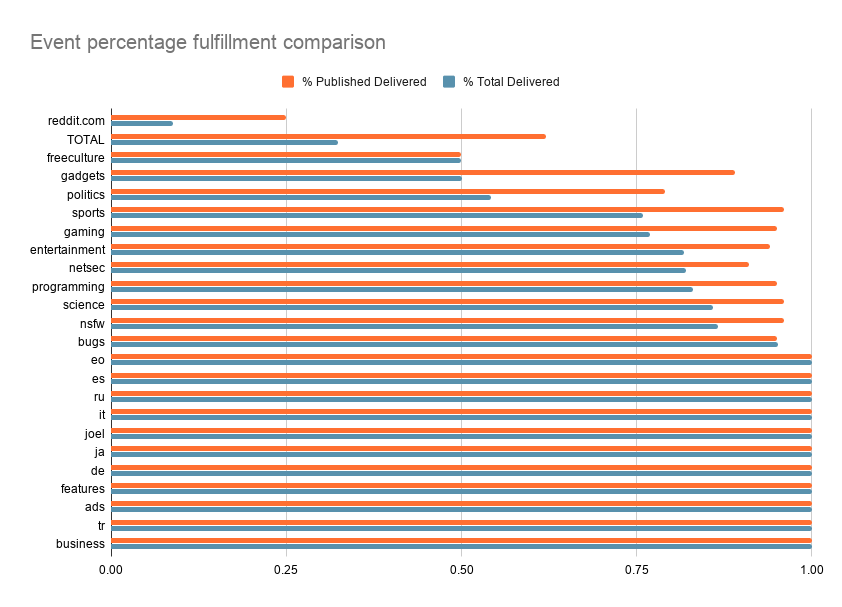
\includegraphics[width=0.4\textwidth]{img/graph-pulsarcast-order-latency-event-percentage-fulfillment-comparison.png}
  \caption{Pulsarcast with order guarantee and latency - Comparison of percentage of events fulfilled by topic}
  \label{fig:graph-pulsarcast-order-latency-event-percentage-fulfillment-comparison}
\end{figure}

It is important to highlight that, for all of the Pulsarcast executions we have
described so far, network and memory usage across the cluster always grew
linearly with the number of events received. Same for the RPC messages sent and
received, as we can see from Figure \ref{fig:graph-pulsarcast-rpc}

\begin{figure}[!htb]
  \centering
  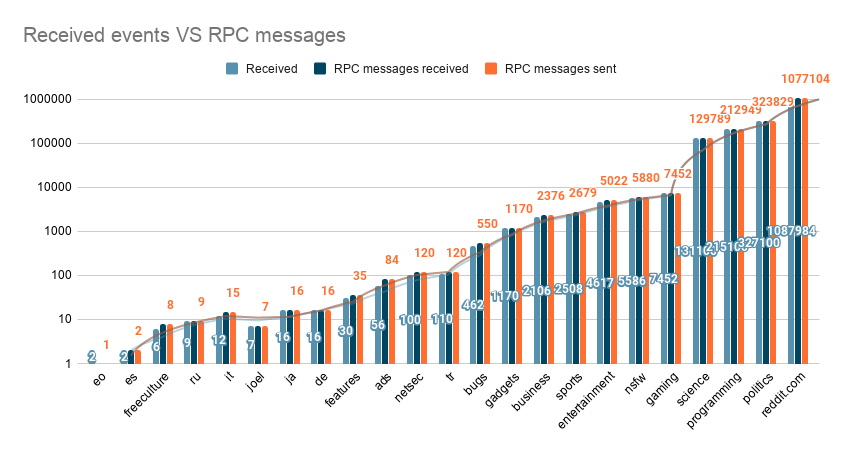
\includegraphics[width=0.4\textwidth]{img/graph-pulsarcast-rpc.png}
  \caption{Pulsarcast without order guarantee - Comparison of events received and RPC injected in the system}
  \label{fig:graph-pulsarcast-rpc}
\end{figure}

Finally our Floodsub scenario executions gave us the following
results~\footnote{For Floodsub there is no distinction between an event
injected into the system and an event published, given there is no
acknowledgement for it}:

\begin{itemize}
  \item 41\% of subscription coverage under normal network conditions
  \item 31\% of subscription coverage, under abnormal network conditions
\end{itemize}

Figures \ref{fig:graph-floodsub-event-percentage-fulfillment-comparison} and
\ref{fig:graph-floodsub-latency-event-percentage-fulfillment-comparison} show
us a comparison of event fulfilment rates across topics. For both experiments,
the network as a whole was unable to cope with the load of our execution and
shortly after starting, some nodes became unresponsive and were terminated,
going as low as only 15 node running at a given time. It took about 50 minutes
for the network to fully recover to 100 nodes again. This is a clear indicator
of Floodsub's inability to handle the same workload Pulsarcast did in the
previous scenarios. Which is expected, as the way Floodsub operates is by
forwarding messages to all of its peers, creating a huge strain in the network
(both CPU wise and in network data transmission). In terms of resource usage,
memory consumption has been lower than the Pulsarcast experiments,hitting a
maximum of 21.15 GiB for the first experiment and 15.95 for the second one.
However, CPU has been way higher, picking at 5.53 vCPUs across the cluster.
Network wise, Floodsub experiments have transmitted much more data for a lower
QoS level, specifically 6552 MiB and 6474 MiB for both experiments across the
cluster, three times as much for the respective Pulsarcast experiments.

\begin{figure}[!htb]
  \centering
  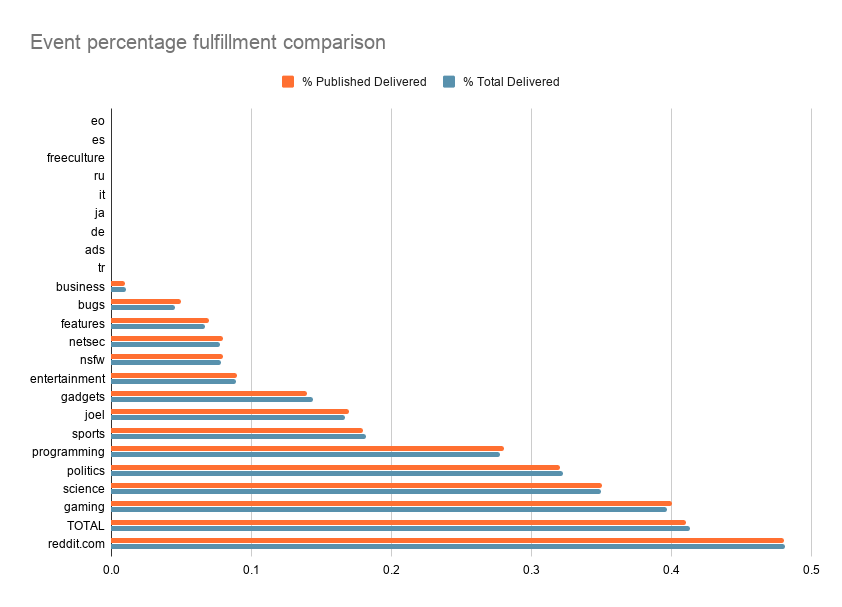
\includegraphics[width=0.4\textwidth]{img/graph-floodsub-event-percentage-fulfillment-comparison.png}
  \caption{Floodsub - Comparison of percentage of events fulfilled by topic}
  \label{fig:graph-floodsub-event-percentage-fulfillment-comparison}
\end{figure}

\begin{figure}[!htb]
  \centering
  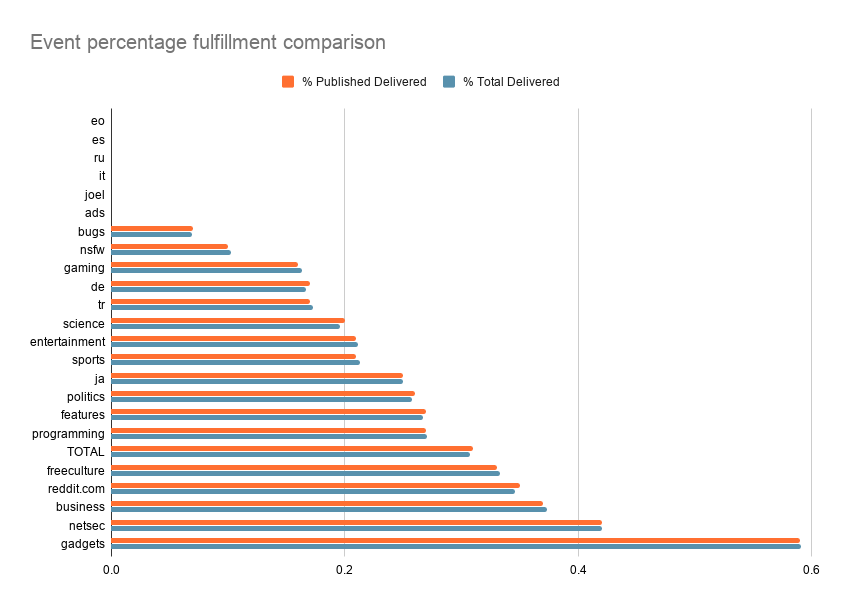
\includegraphics[width=0.4\textwidth]{img/graph-floodsub-latency-event-percentage-fulfillment-comparison.png}
  \caption{Floodsub with latency - Comparison of percentage of events fulfilled by topic}
  \label{fig:graph-floodsub-latency-event-percentage-fulfillment-comparison}
\end{figure}

One aspect that we would like to highlight is the fact that we are not only
compressing months of data into a largely shorter timepsan, we are also
simulating interactions made by thousands of users into a much smaller set of
nodes (one hundred). All of this of course in an environment based on
virtualisation techniques and with a limited set of resources. This experiment
is essentially pushing the boundaries of what both systems would handle on a
real world scenario. Equally important to note is that, for Pulsarcast, every
event effectively published, is stored in the DHT. So, it is possible for any
application using Pulsarcast to resolve past or missing events from the event
tree. This is the cornerstone of Pulsarcast's eventual delivery guarantees,
hence why it is essential to look at the percentage of events effectively
published as well as the subscription coverage for these same events. Taking
those same numbers into consideration we can see a considerably high coverage
percentage, with the lowest being 62\% for the order guarantee test with
latency injected.
